% =============================================================================
% Deleted-Record Recovery from SQLite Databases
% A reference implementation and a multi-oracle forensic evaluation
% XeLaTeX + xeCJK, two-column
% Build: xelatex -> bibtex -> xelatex x2   (see Makefile)
% =============================================================================
\documentclass[10pt,a4paper]{article}

% --- Packages ----------------------------------------------------------------
\usepackage{fontspec}
\usepackage{xeCJK}
\setCJKmainfont{Songti TC}
\setCJKsansfont{Songti TC}
\setCJKmonofont{Songti TC}
\usepackage{amsmath,amssymb,amsfonts}
\usepackage{booktabs}
\usepackage{multirow}
\usepackage{graphicx}
\usepackage{xcolor}
\usepackage{hyperref}
\usepackage[margin=0.75in]{geometry}
\usepackage{enumitem}
\usepackage{float}
\usepackage{caption}
\usepackage{subcaption}
\usepackage{siunitx}
\usepackage{longtable}
\usepackage[numbers,sort&compress]{natbib}
\usepackage{xurl}
\usepackage{authblk}
\usepackage{pgfplots}
\usepackage{tikz}
\usepackage{textcomp}
\usepackage{adjustbox}
\usepackage[framemethod=tikz]{mdframed}

\pgfplotsset{compat=1.18}

\setlength{\columnsep}{18pt}
\setlength{\emergencystretch}{3em}

\hypersetup{
    colorlinks=true,
    linkcolor=blue!70!black,
    citecolor=green!50!black,
    urlcolor=blue!60!black,
}

\newcommand{\zh}[1]{#1}
\newcommand{\orcidlink}[1]{%
  \href{https://orcid.org/#1}{\textcolor{green!50!black}{\textsf{iD}}}%
}
\newcommand{\code}[1]{\texttt{#1}}

\newmdenv[
  linecolor=gray!50, linewidth=0.4pt, backgroundcolor=gray!4,
  skipabove=6pt, skipbelow=6pt, innertopmargin=5pt, innerbottommargin=5pt,
]{fnote}

\definecolor{ours}{HTML}{1B9E8A}
\definecolor{fqlitec}{HTML}{E6840F}
\definecolor{undarkc}{HTML}{D62728}
\definecolor{bring}{HTML}{7570B3}

% --- Title -------------------------------------------------------------------
\title{%
  \textbf{Deleted-Record Recovery from SQLite Databases:}\\[4pt]
  \large Storage Conventions, a \texttt{forbid(unsafe)} Reference Implementation,\\
  and a Multi-Oracle Forensic Evaluation%
}

\author[1]{Albert Kwun Tai Hui\,\orcidlink{0009-0000-8978-0231}}
\affil[1]{Security Ronin}

\date{June 2026}

% =============================================================================
\begin{document}

\twocolumn[
\maketitle

\begin{abstract}
SQLite is the most widely deployed database engine in the world~\cite{sqlite_mostdeployed},
and the deleted rows inside its files are routinely the evidence an investigator
needs---yet the live query interface (\code{sqlite3}) cannot see them. This paper
gives an end-to-end account of where deleted data persists in a SQLite file and
how to recover it defensibly. We set out the storage model and the conventions
that govern residue lifetime: the comparative retirement of the rollback
\code{-journal} in application contexts in favour of the write-ahead log
(\code{-wal}, which retains \emph{multiple} uncheckpointed commits), and the
destructive effect of \code{VACUUM} and \code{PRAGMA secure\_delete}. We then
describe a complete set of recovery mechanisms---freelist and free-block carving,
exact-tile free-block reconstruction, overflow-chain reassembly, dropped-table
schema recovery, a WAL commit-history overlay, and rollback-journal before-image
folding---unified under a structural \emph{never re-read a live row}
(false-positive-zero) guarantee enforced by construction rather than by heuristic.

We contribute: (1)~a systematic treatment of SQLite deletion and free-space
conventions, including an application case study of \zh{微信} (WeChat) message
deletion; (2)~\code{sqlite4n6}, an open, \code{forbid(unsafe)} Rust reference
implementation; and (3)~a multi-oracle evaluation---accuracy, false-positive
rate, and throughput---against four independent recovery tools (\code{undark},
\code{fqlite}, \code{bring2lite}, and the SQLite Deleted-Records Parser) on
independent third-party corpora with published ground truth. On the in-page
deletion category of the Nemetz standardized corpus our recall leads the strongest
competitor (0.833 vs.\ 0.798) at precision 1.000 with zero live-row re-reads;
across the whole evaluated corpus we re-surface \emph{no} still-live row. Every
figure is reproducible from the cited artifacts.
\end{abstract}
\vspace{12pt}
]

% === §1 Introduction =========================================================
\section{Introduction}\label{sec:intro}

SQLite ships inside every major browser, mobile operating system, and messaging
application, making a SQLite file among the most common artifacts in a digital
investigation~\cite{sqlite_mostdeployed}. The records a custodian \emph{deleted}---a
cleared chat, a removed history entry, a purged transaction---are frequently the
records that matter, and they often still reside, intact or partially intact, in
the file's free space, in an uncheckpointed write-ahead log, or in a rollback
journal. The ordinary access path cannot reach them: \code{sqlite3} and the
language bindings traverse the \emph{live} b-tree and stop, by design.

Recovering that residue is a mature subfield. Nemetz \emph{et al.} published a
standardized corpus and showed that no single tool reliably handles all
SQLite corner cases~\cite{nemetz2018corpus}; Pawlaszczyk and
Hummert~\cite{pawlaszczyk2021fqlite} and Meng and Baier~\cite{meng2019bring2lite}
contributed carving tools and techniques; and the recent survey of Lee, Park, Lee
and Choi~\cite{choi2025survey} organizes the field into three families of
technique---metadata-based, carving-based, and WAL-based recovery---and evaluates
representative open-source tools on recovery rate, reliability, and false
positives. Two gaps motivate this work. First, the literature treats the storage
\emph{conventions} that decide whether residue exists at all---WAL versus
rollback journaling, \code{VACUUM}, and \code{secure\_delete}---unevenly, even
though they dominate real-case outcomes. Second, recovery tools differ sharply in
whether they ever mistake a \emph{live} row for a deleted one, and that
false-positive behaviour is rarely guaranteed structurally.

This paper addresses both. We give a precise account of the storage model and the
conventions (\S\ref{sec:storage}--\S\ref{sec:conventions}); we describe a full set
of recovery mechanisms (\S\ref{sec:mechanisms}) under a structural
false-positive-zero design (\S\ref{sec:fpzero}); we present an open reference
implementation (\S\ref{sec:impl}); and we evaluate it against four independent
oracles on third-party corpora with published ground truth
(\S\ref{sec:corpus}--\S\ref{sec:eval}).

\subsection*{Contributions}
\begin{enumerate}[leftmargin=1.4em,itemsep=2pt]
  \item A systematic account of SQLite's on-disk deletion behaviour and the
        free-space lifetime conventions (journal vs.\ WAL, \code{VACUUM},
        \code{secure\_delete}), with an application case study of WeChat
        (\S\ref{sec:storage}--\S\ref{sec:conventions}).
  \item A structural false-positive-zero recovery design and an open,
        \code{forbid(unsafe)} reference implementation, \code{sqlite4n6}
        (\S\ref{sec:fpzero}--\S\ref{sec:impl}).
  \item A reproducible multi-oracle evaluation---accuracy, false positives, and
        throughput---on independent corpora with published ground truth
        (\S\ref{sec:corpus}--\S\ref{sec:eval}).
\end{enumerate}

% === §2 The SQLite storage model =============================================
\section{Where Deleted Data Lives}\label{sec:storage}

The SQLite database file is a sequence of fixed-size \emph{pages}~\cite{sqlite_fileformat}.
A table is a b-tree whose leaf pages hold \emph{cells}, one per row; each cell is a
varint-prefixed record of serial-typed values keyed by an integer \code{rowid}.
Recovery hinges on what happens to a cell's bytes once the row is no longer
reachable from the b-tree.

\subsection*{Free blocks and the freelist}
When a row is deleted, SQLite does not erase its bytes. The cell is unlinked from
the page's cell-pointer array, and its span is either added to that page's
intra-page \emph{free-block} chain---a linked list of freed gaps inside an
otherwise live page---or, when a page empties completely, the page is placed on the
database \emph{freelist} of reusable pages~\cite{sqlite_fileformat}. In both cases
the original record bytes survive until that space is next \emph{allocated} and
overwritten. That window is what every carving technique exploits. A freed cell's
first bytes (the leading payload-length and rowid varints) may be partly
overwritten by the free-block header that now occupies the gap; the surviving tail
still carries the record's serial-type array and values.

\subsection*{Overflow pages}
A value too large for one page spills onto a chain of \emph{overflow} pages linked
by a four-byte next-page pointer~\cite{sqlite_fileformat}. A deleted row with a long
\code{TEXT} or \code{BLOB} column therefore leaves residue spread across several
pages---recoverable only by following, or reconstructing, the chain through the
freelist.

\subsection*{The rollback journal and the write-ahead log}
SQLite offers two crash-recovery mechanisms, and each leaves a distinct,
recoverable side file. The \emph{rollback journal} (\code{<db>-journal}) holds the
\emph{before}-images of pages a transaction is about to modify, so that an aborted
transaction can be rolled back. The \emph{write-ahead log} (\code{<db>-wal}),
available since SQLite 3.7.0 (2010)~\cite{sqlite_wal}, inverts this: new page
versions are \emph{appended} to the WAL and only later \emph{checkpointed} back
into the main file. The two files are temporal mirror images---the journal holds
the pre-transaction state, the WAL the post-transaction states---and both are
forensically rich.

\begin{fnote}\small
\textbf{A \code{-wal} holds many commits.} A WAL begins with a 32-byte header (a
magic number, the page size, and two random \emph{salt} values) followed by
\emph{frames}, each a 24-byte frame-header plus one page image. A frame whose
header carries a non-zero ``database size in pages'' field is a \emph{commit}
marker; a single WAL ``can and usually does record multiple
transactions''~\cite{sqlite_wal}. The salts are copied into every frame and
re-randomized per transaction so stale frames from a previous journal cannot be
mistaken for current ones. Checkpointing is automatic once the WAL reaches a
threshold (1000 pages by default)~\cite{sqlite_wal}. Until then, the WAL retains
the \emph{commit history}: a page version a later commit superseded, or a row a
later commit deleted, survives in the earlier frames.
\end{fnote}

% === §3 Deletion conventions in practice =====================================
\section{Conventions That Govern Residue}\label{sec:conventions}

Whether deleted data is recoverable at all is decided less by the deletion itself
than by three conventions: which journaling mode the application uses, whether
\code{VACUUM} has run, and whether \code{secure\_delete} is enabled.

\subsection*{Rollback journaling vs.\ WAL}
SQLite's \emph{library} default remains rollback journaling in \code{DELETE} mode
(the journal file is deleted at commit); the other rollback modes are
\code{TRUNCATE}, \code{PERSIST} (the journal is kept but its header
zeroed), \code{MEMORY}, and \code{OFF}~\cite{sqlite_pragma}. Many modern
applications, however, \emph{opt into} WAL mode for concurrency, so in practice a
\code{-wal} sidecar is the common case for mobile and desktop application
databases while a persistent \code{-journal} is comparatively legacy. The
distinction matters forensically: a \code{DELETE}-mode journal is removed at
commit and leaves nothing on a clean shutdown, whereas a \code{PERSIST} journal or
an uncheckpointed WAL is a durable record of prior state---and the WAL, holding
\emph{multiple} commits, is the richer of the two.

\subsection*{\code{VACUUM} is anti-forensic}
\code{VACUUM} ``rebuilds the database file, repacking it into a minimal amount of
disk space''~\cite{sqlite_vacuum}. In doing so it discards the freelist and the
free-block slack that carving relies on. The SQLite documentation is explicit:
deleted content ``can allow deleted content to be recovered \dots\ Running
\code{VACUUM} will clean the database of all traces of deleted content, thus
preventing an adversary from recovering deleted content''~\cite{sqlite_vacuum}. A
vacuumed database is, for residue purposes, scrubbed. \code{auto\_vacuum}
incrementally reclaims emptied pages but ``does not compact partially filled
pages''~\cite{sqlite_pragma}, so it destroys whole-page freelist residue while
leaving intra-page free-block residue.

\subsection*{\code{PRAGMA secure\_delete}}
With \code{secure\_delete=ON}, SQLite overwrites freed content with zeros at
deletion time, eliminating residue; it is \emph{off} by default, and a
later \code{FAST} variant zeroes content only when doing so adds no
I/O~\cite{sqlite_pragma}. An investigator must therefore treat the presence of
recoverable residue as evidence that \code{secure\_delete} was \emph{not} in
force---and its absence as inconclusive rather than as proof of secure deletion.

\subsection*{Application case study: \zh{微信} (WeChat)}
WeChat, the dominant Chinese super-app, illustrates how application conventions
shape recovery. On Android, chat history is stored in an SQLCipher-encrypted
database \code{EnMicroMsg.db} (messages in the \code{message} table, contacts in
\code{rcontact}); on iOS the store is \code{MM.sqlite}, often
unencrypted~\cite{hur2020wechat}. The Android database key is derived as the first
seven hexadecimal characters of \code{MD5(IMEI\,\textbar\textbar\,UIN)}~\cite{hur2020wechat}.
Hur \emph{et al.} show that deleted WeChat messages can be recovered from the
tokenized index of the full-text-search database (\code{FTS5IndexMicroMsg.db})
even after the message row is gone, and give a decryption method for the
IMEI-absent case (Wi-Fi-only tablets); they further note that attachment metadata
persists in the \code{appattach} table after deletion and that deletions are not
synchronized across the Android and Windows clients, so a message purged on one may
survive on the other~\cite{hur2020wechat}. The recovery techniques in this
paper apply once such a database is decrypted to plaintext SQLite: the deleted
rows live in the same free blocks, overflow chains, and WAL frames as any other
SQLite artifact.

% === §4 Recovery mechanisms ==================================================
\section{Recovery Mechanisms}\label{sec:mechanisms}

We implement the three technique families of the Choi survey~\cite{choi2025survey}
---metadata-based, carving-based, and WAL-based---as the following mechanisms.
Each emits a labelled \emph{recovery source} and a confidence
(\S\ref{sec:fpzero}); each preserves the live-row invariant by construction.

\paragraph{Free-block and freelist carving (metadata- and carving-based).}
Whole pages on the freelist contain only deallocated content and are the strongest
case; intra-page free blocks are gaps in still-live pages and are more likely to be
partly overwritten. We carve both, decoding each candidate cell against the live
schema and reading every value in its native serial type.

\paragraph{Exact-tile free-block reconstruction.}
When a freed cell's leading bytes are destroyed by the free-block header, the cell
length and \code{rowid} are gone but the serial-type tail survives. We rebuild the
record from the surviving tail plus the owning table's schema template, accepting a
reconstruction only when it \emph{exactly tiles} the free block---its decoded
extent must end precisely on the block boundary. This exactness gate is what
rejects column-shifted phantoms, and it extends to two-byte \code{rowid}s
($\geq 128$) and to runs of coalesced freed cells, where each cell in the span must
tile in turn. The destroyed \code{rowid} is surfaced as absent rather than guessed.

\paragraph{Overflow-chain reassembly (carving-based).}
A deleted row whose payload spilled onto overflow pages is reassembled by following
the freed chain through the freelist leaves to a byte-exact body. Because a freelist
leaf can be stale, this path is graded below an intact in-page cell.

\paragraph{Dropped-table schema recovery (metadata-based).}
A dropped table's definition survives as a deleted \code{sqlite\_master} row in
page-1 free space. We recover the dropped table, index, view, or trigger name and
its \code{CREATE} statement, which both documents the deletion and supplies a
schema template for attributing other residue.

\paragraph{The WAL commit-history overlay (WAL-based).}
We parse the WAL frame by frame, reconstruct the database state at each
\code{COMMIT} marker, and surface rows that were live at an earlier commit but
deleted by a later one. Each recovered version carries its log-sequence provenance
(the two salts and the frame index), giving an ordered edit history rather than a
flat dump. There is no wall-clock timestamp in a WAL---only this commit order.

\paragraph{Rollback-journal before-image folding (WAL-based, temporal inverse).}
When a \code{<db>-journal} is present we fold in the \emph{before}-images of the
last transaction: rows it deleted and the pre-edit values of rows it modified. This
is the temporal inverse of the WAL---where the WAL holds after-images, the journal
holds the before-image of the last transaction.

\paragraph{Tier-2 fragment salvage.}
Where a full row cannot be reconstructed but a \emph{distinctive} cell survives at a
structural anchor (a \code{TEXT} value of at least four UTF-8 bytes, or a
\code{REAL}), we salvage the maximal decodable column prefix as a \emph{fragment}---a
typed object with no \code{rowid} and an incomplete column set, kept in a separate
output surface so it can never be mistaken for a full recovered row.

% === §5 The false-positive-zero guarantee ====================================
\section{Never Re-Reading a Live Row}\label{sec:fpzero}

In a forensic setting, reporting a still-\emph{live} row as ``deleted'' is the
costliest error: it fabricates evidence. Our design makes that outcome structurally
impossible, in two layers.

\paragraph{Structural exclusion.} We first compute the byte extents of every
\emph{live} cell directly from the b-tree structure. The set of carvable free
regions is then defined as the \emph{complement} of those extents within each page.
Carving runs only inside free regions, so a row still reachable from the live
b-tree is never scanned for recovery in the first place.

\paragraph{Value-collision filter.} A freed cell's bytes can, in principle,
coincide with a live row's values (for example, a freed copy left by an in-place
\code{UPDATE}). After carving, any recovered record whose decoded values equal those
of a live row in the same table is dropped. What remains---an \code{UPDATE}'s freed
\emph{prior} version, whose values differ from the live row---is genuine deleted
edit history, not a duplicate.

These two layers are independent of confidence: a still-live row is excluded
regardless of any threshold. Confidence, by contrast, manages \emph{phantoms}
(coincidental byte sequences that decode to a plausible but spurious record), and
is reported, never used to suppress a live-row collision.

\paragraph{Confidence model.} Every recovered item carries a confidence set by its
recovery path (Table~\ref{tab:confidence}). A base of $0.9$ for a full row with
distinctive text is attenuated by an in-page factor ($0.8$) for free-block residue
and by an overflow-chain factor ($0.75$) for chain-reassembled bodies; freeblock
reconstructions take a fixed $0.4$ and fragments $0.2$. The CLI exposes a
\code{-{}-min-confidence} ladder (\code{info}\,$0.0$, \code{low}\,$0.2$,
\code{medium}\,$0.4$, \code{high}\,$0.6$, \code{critical}\,$0.8$) that filters
every emitted item; it is a recall/noise dial, not a safety control.

\begin{table}[t]
\centering\small
\caption{Confidence assigned by recovery path.}
\label{tab:confidence}
\begin{tabular}{@{}c p{0.60\columnwidth}@{}}
\toprule
Conf. & Recovery path \\
\midrule
$0.9$   & full row, distinctive text (freelist / WAL frame / live-anchor) \\
$0.72$  & in-page free block, distinctive text ($0.9\times0.8$) \\
$0.675$ & overflow-chain reassembly ($0.9\times0.75$) \\
$0.6$   & full row, no distinctive text \\
$0.48$  & in-page free block, no distinctive text ($0.6\times0.8$) \\
$0.4$   & exact-tile free-block reconstruction \\
$0.3$   & free-block reconstruction spilling to overflow ($0.4\times0.75$) \\
$0.2$   & Tier-2 fragment \\
\bottomrule
\end{tabular}
\end{table}

% === §6 Reference implementation =============================================
\section{Reference Implementation}\label{sec:impl}

\code{sqlite4n6} is an open-source Rust workspace of three crates: \code{sqlite-core}
(a panic-free, read-only file-format reader: b-tree, WAL, freelist, overflow),
\code{sqlite-forensic} (the carving and audit harness with the recovery oracles),
and \code{sqlite4n6} (the command-line tool). All three are \code{forbid(unsafe)};
the project pins a current Rust toolchain, declares a conservative minimum
supported version, and gates on \SI{100}{\percent} function coverage in continuous
integration. The reader opens evidence \emph{read-only} and, for WAL artifacts,
in immutable mode, so analysis never mutates or checkpoints the file under
examination.

Output is designed for review rather than for re-parsing. The default carve writes
a per-rowid \emph{version-history} workbook---live rows interleaved with the prior
and deleted versions recovered from the WAL, the rollback journal, and free space,
ordered by commit sequence and tinted by state---with image BLOBs rendered as
in-cell thumbnails. A \code{-f db} option emits a queryable SQLite database whose
recovered rows are attributed in three honest tiers (observed fact, forensic
inference, unknown), and \code{-f jsonl}/\code{csv} stream the raw records. Every
record carries provenance columns: page, byte offset, \code{rowid} (or absent),
recovery source, and confidence.

% === §7 Validation corpus ====================================================
\section{Validation Corpus}\label{sec:corpus}

A recovery tool validated only against fixtures its own authors built inherits
their blind spots. We therefore validate primarily against third-party corpora
whose \emph{ground truth was authored by someone else}, and label every result by
the strength of the check that vouches for it (Table~\ref{tab:tiers}).

\begin{table*}[t]
\centering\small
\caption{Evidence tiers. Tier~1 = an independent party authored both the artifact
and the answer key (or it is real-device data); Tier~2 = real \code{sqlite3}-engine
bytes whose ground truth is derivable from the documented construction or confirmed
by an independent oracle; Tier~3 = authored by us with nothing independent vouching.}
\label{tab:tiers}
\begin{tabular}{@{}l p{0.40\textwidth} p{0.42\textwidth}@{}}
\toprule
Tier & Corpus / oracle & What it establishes \\
\midrule
1 & Nemetz standardized corpus~\cite{nemetz2018corpus} (141 DBs, CC0, per-row \code{.xml} keys) & deleted-record recall \& precision vs.\ third-party ground truth \\
1 & NIST CFReDS / CFTT SQLite sets~\cite{nist_cfreds_sqlite} (SFT-01/03/05) & text encodings; WAL \& journal recovery; native types + BLOBs \\
1 & NIST CFReDS \emph{Data Leakage} (\code{snapshot.db} from a Volume Shadow Copy) & real-case end-to-end recovery of two deleted rows, one freeblock-clobbered \\
1 & DC3 \code{sqlite\_dissect} corpus~\cite{sqlite_dissect_dc3} (no-deletion baseline) & zero false positives on unallocated content \\
1 & \code{sqlite-unhide} corpus (9 DBs, independent \code{.txt} keys) & two-byte-rowid free-block recovery; surfaced two real defects \\
1 & Josh Hickman iOS-17 images (genuine app databases) & no-panic robustness over real device data \\
2 & real-\code{sqlite3} fixtures; \code{sqlite3 .recover}; \code{calamine} XLSX reader & construction-derivable answers; differential agreement; output round-trip \\
\bottomrule
\end{tabular}
\end{table*}

The head-to-head accuracy results below use the Nemetz standardized
corpus~\cite{nemetz2018corpus}, whose authors published a per-row answer key for
every deleted record. We score the three deletion categories with a format-stable
identity (in-page deletion \code{0C}, deleted-then-overwritten \code{0D}, and
deleted overflow \code{0E}); categories whose only key column is a floating-point
value rendered differently by each tool are excluded from the cross-tool key, as
are the whole-table-loss and anti-forensic categories that have no deleted-row
anchor.

% === §8 Evaluation ===========================================================
\section{Evaluation}\label{sec:eval}

\subsection*{Accuracy: a multi-oracle head-to-head}
We compare \code{sqlite4n6} against four independent recovery tools---\code{undark}
(C)~\cite{undark}, \code{fqlite} (Java)~\cite{pawlaszczyk2021fqlite}, \code{bring2lite}
(Python)~\cite{meng2019bring2lite}, and the SQLite Deleted-Records Parser
(SQL-DRP, Python)~\cite{degrazia_sqlparse}---each scored against the \emph{same}
Nemetz answer key with the same two-column identity matcher
(Table~\ref{tab:headtohead}). Recall is computed on the substrate of rows whose
identity still survives in the artifact; precision counts phantom rows; the
``live'' column counts still-live rows wrongly reported as deleted. \code{fqlite}
is driven through a headless source-instrumentation tap of its carving engine; the
two Python tools through normalizing wrappers. The patches, shims, and exact
versions are committed so the comparison is independently reproducible.

\begin{table}[t]
\centering\small
\caption{Deleted-record recovery on the Nemetz corpus (categories \code{0C}/\code{0D}/\code{0E};
$D_{\mathrm{rec}}$ = recoverable-substrate denominator). All recall/TP figures are
harness-computed against the published answer key. \code{fqlite}'s precision is
measured through our committed headless tap.}
\label{tab:headtohead}
\setlength{\tabcolsep}{4pt}
\begin{tabular}{@{}llrrrrr@{}}
\toprule
Cat & Tool & TP & FP & FN & Rec. & Prec. \\
\midrule
\multirow{5}{*}{\code{0C}}
 & \textbf{ours}   & \textbf{70} & \textbf{0}  & 14 & \textbf{0.833} & \textbf{1.000} \\
 & fqlite          & 67 & 17 & 17 & 0.798 & 0.798 \\
 & bring2lite      & 40 & 0  & 44 & 0.476 & 1.000 \\
 & undark          & 14 & 10 & 70 & 0.167 & 0.583 \\
 & sql-drp         & 0  & 1  & 84 & 0.000 & 0.000 \\
\midrule
\multirow{5}{*}{\code{0D}}
 & \textbf{ours}   & 19 & 0 & 0 & \textbf{1.000} & \textbf{1.000} \\
 & fqlite          & 20 & 0 & 0 & 1.000 & 1.000 \\
 & bring2lite      & 7  & 0 & 12 & 0.368 & 1.000 \\
 & undark          & 1  & 10 & 18 & 0.053 & 0.091 \\
 & sql-drp         & 0  & 0 & 19 & 0.000 & --- \\
\midrule
\multirow{5}{*}{\code{0E}}
 & \textbf{ours}   & \textbf{4} & \textbf{0} & 0 & \textbf{1.000} & \textbf{1.000} \\
 & undark          & 3 & 6 & 1 & 0.750 & 0.333 \\
 & bring2lite      & 3 & 5 & 1 & 0.750 & 0.375 \\
 & fqlite          & 2 & 6 & 2 & 0.500 & 0.250 \\
 & sql-drp         & 0 & 0 & 4 & 0.000 & --- \\
\bottomrule
\end{tabular}
\end{table}

On in-page deletion (\code{0C}) our carver recovers 70 of 84 recoverable rows
(recall $0.833$) ahead of \code{fqlite}'s 67 ($0.798$), and does so at precision
$1.000$---zero phantom rows and zero live re-reads---against \code{fqlite}'s
$0.798$. On deleted-then-overwritten rows (\code{0D}) our carver and \code{fqlite}
both recover every row whose full identity survives, at precision $1.000$; on the
small overflow substrate (\code{0E}) our carver recovers all four at precision
$1.000$, including one reassembled overflow chain. Across the evaluated corpus our
carver re-surfaces \emph{no} still-live row; \code{undark}, which dumps live and
deleted rows together, re-reads 56 live rows as deleted on \code{0D} alone.
Figure~\ref{fig:pr} plots the precision--recall plane.

\begin{figure}[t]
\centering
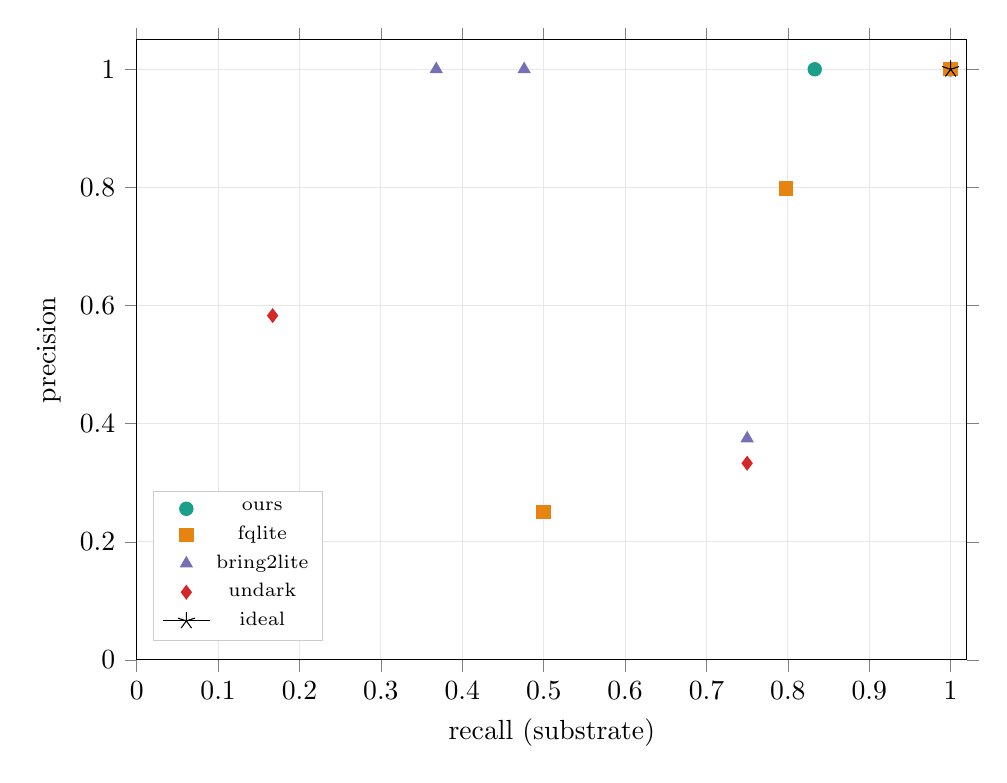
\begin{tikzpicture}
\begin{axis}[
  width=\columnwidth, height=0.78\columnwidth,
  xlabel={recall (substrate)}, ylabel={precision},
  xmin=0, xmax=1.02, ymin=0, ymax=1.05,
  grid=both, grid style={gray!18}, tick align=outside,
  legend style={at={(0.02,0.03)}, anchor=south west, font=\scriptsize, draw=gray!40},
  mark size=2.4pt,
]
% ours
\addplot[only marks, mark=*, ours] coordinates {(0.833,1.0) (1.0,1.0) (1.0,1.0)};
\addlegendentry{ours}
% fqlite
\addplot[only marks, mark=square*, fqlitec] coordinates {(0.798,0.798) (1.0,1.0) (0.5,0.25)};
\addlegendentry{fqlite}
% bring2lite
\addplot[only marks, mark=triangle*, bring] coordinates {(0.476,1.0) (0.368,1.0) (0.75,0.375)};
\addlegendentry{bring2lite}
% undark
\addplot[only marks, mark=diamond*, undarkc] coordinates {(0.167,0.583) (0.053,0.091) (0.75,0.333)};
\addlegendentry{undark}
\addplot[mark=star, mark size=3.2pt, black] coordinates {(1.0,1.0)};
\addlegendentry{ideal}
\end{axis}
\end{tikzpicture}
\caption{Precision--recall across categories \code{0C}/\code{0D}/\code{0E}
(SQL-DRP omitted: it recovers no answer-key row under the format-stable identity).
Our carver sits on the precision-1.0 ceiling in every category.}
\label{fig:pr}
\end{figure}

\subsection*{False positives across forensic hazards}
Accuracy on a clean corpus says little about the hazard that matters most---mistaking
live data for deleted. We replicate the three adversarial scenarios of the Choi
survey~\cite{choi2025survey} on real \code{sqlite3}-engine bytes (a Tier-2
\emph{replication} of the published construction, not the authors' own files):
\code{0F}, where a b-tree rebalance moves a live row onto a freed page; \code{0B},
a drop-and-recreate of a same-schema table; and \code{10}, a \code{secure\_delete}
wipe of the main image leaving residue only in the WAL. On \code{0F},
\code{sqlite4n6} recovers 33 of 50 with \emph{zero} live false positives, where
\code{bring2lite} re-surfaces 13 live rows; on \code{10}, the WAL-only scenario,
both WAL-aware tools recover all 20, while the main-image-only tools recover none.

\subsection*{Throughput}
On a generated \SI{100}{\mega\byte} database with 80{,}000 deleted rows
(single machine, median of five runs), \code{sqlite4n6} streaming JSONL recovers
79{,}904 deleted rows (recall $0.9988$) with zero live false positives in
\SI{15.6}{\second}. The faster tools do different work: \code{undark} dumps
177{,}906 rows---live and deleted together, undifferentiated---in
\SI{1.5}{\second}, and SQL-DRP emits 5 printable-string carves in
\SI{0.2}{\second}. Throughput is therefore not directly comparable across tools
that recover different things; we report it for completeness, not as a headline.

% === §9 Related work =========================================================
\section{Related Work}\label{sec:related}

The Choi survey~\cite{choi2025survey} is the closest prior work: it organizes
SQLite deleted-record recovery into metadata-based, carving-based, and WAL-based
families and evaluates the same open-source tools we compare against, with explicit
attention to false positives. We extend it with a structural false-positive-zero
\emph{guarantee} and a reproducible head-to-head on the standardized corpus.
Nemetz \emph{et al.}~\cite{nemetz2018corpus} contributed the standardized corpus
and the finding that no tool handles every corner case---which our multi-oracle
evaluation re-confirms tool by tool. \code{fqlite}~\cite{pawlaszczyk2021fqlite} and
\code{bring2lite}~\cite{meng2019bring2lite} are the strongest open carvers and
recover free-block and freelist residue; \code{undark}~\cite{undark} dumps all
intact records without separating live from deleted; SQL-DRP~\cite{degrazia_sqlparse}
carves printable strings from freed regions; and DC3's
\code{sqlite\_dissect}~\cite{sqlite_dissect_dc3} parses the database together with
its journal and WAL. On the application side, Hur \emph{et al.}~\cite{hur2020wechat}
recover deleted WeChat messages from full-text-search index residue, complementary
to the free-space and WAL recovery treated here.

% === §10 Discussion ==========================================================
\section{Discussion and Limitations}\label{sec:discussion}

Recovery is bounded by the conventions of \S\ref{sec:conventions}: \code{VACUUM}
and \code{secure\_delete} destroy residue, and an allocation that overwrites a
freed cell ends its recoverability. Our end-to-end recall on overflow bodies is
low ($0.333$ on \code{0E}) precisely because most deleted overflow payloads in the
corpus were genuinely overwritten---an honest ceiling, not a defect, and one our
substrate recall of $1.000$ makes explicit. The competitor precision figures we
report are measured through our own headless taps and wrappers; recall, the
substantive engine result, reproduces exactly, while a tool's phantom count depends
on its emission policy, which we re-derived for \code{fqlite}. Finally, our
false-positive scenarios are a replication of the Choi survey's construction on
real-engine bytes rather than the authors' own files; we label them Tier-2
accordingly.

% === §11 Conclusion ==========================================================
\section{Conclusion}\label{sec:conclusion}

Deleted SQLite records persist in free blocks, overflow chains, rollback journals,
and---most richly---in the multiple uncheckpointed commits of a write-ahead log,
until \code{VACUUM}, \code{secure\_delete}, or reallocation erases them. We have
described a complete set of recovery mechanisms for that residue, unified by a
structural guarantee that a still-live row is never reported as deleted, and an
open \code{forbid(unsafe)} reference implementation. Measured against four
independent tools on third-party corpora with published ground truth, the
implementation leads on in-page recall at precision $1.000$ and re-surfaces no live
row across the evaluated corpus. Every number is reproducible from the cited
artifacts.

% =============================================================================
\bibliographystyle{unsrtnat}
\bibliography{sqlite-recovery}

\end{document}
